
\chapter{\IfLanguageName{dutch}{Proof of concept}{Proof of concept}}%
\label{ch:poc}

Aan de hand van de shortlist die opgemaakt is komt er voor elke geselecteerde managementplatform een proof of concept. Hierbij wordt er gekeken hoe de nodige functionaliteiten werken en toegepast kunnen worden in het systeem.
Belangrijk om te weten is dat de proof of concept niet de volledige functionaliteit van het managementplatform zal testen. Het doel is om een goed beeld te krijgen van de mogelijkheden en hoe deze kunnen worden toegepast binnen de infrastructuur van Excentis. 
We verdelen alle managementplatformen in hun eigen subsecties. In deze subsecties worden dan de vooropgestelde testen op uitgevoerd.
\section{Proxmox VE}%
Voor deze virtual managementplatform wordt er Proxmox VE 8.4 gebruikt. Dit is de laatste versie van Proxmox VE die op dit moment beschikbaar is.
\subsection{Storage in Proxmox VE}
Ìn deze proof of concept worden er 2 storage integraties bekeken en getest.
\begin{itemize}
    \item CEPH storage
    \item SAN iSCSI (met TrueNAS ~\autocite{truenas})
\end{itemize}
In sectie \nameref{sec:storage_proxmox} wordt er dieper ingegaan op de configuratie van de storage in Proxmox VE.
CEPH wordt toegepast op alle 3 de fysieke nodes. Elk hebben hun eigen schijf die gebruikt wordt door CEPH. Deze schijven nemen elkaars taken over bij een failover of het maken van redunante data.
iSCI bij Proxmox VE biedt op een makelijke manier de mogelijkheid om een SAN te configureren. 
Beiden werden probleemloos geconfigureerd en getest bij een virtuele machine. Zie \nameref{sec:storage_proxmox} voor meer details.
\subsection{High Availability in Proxmox VE}
In \nameref{sec:ha-proxmox} wordt de configuratie voor HA in detail uitgelgd.
De test zellf wordt uitgevoerd bij 2 virtuele machines die elk gekoppeld zijn aan hun eigen storage systeem (iscsi of CEPH).
Hierna worden ze toegevoegd aan een HA-groep. Dit is een groep van virtuele machines die samen prioriteit hebben in de cluster.

Om HA te testen in combinatie met beide storage systemen zal er een netwerk probleem worden gesimuleerd.
Alle virtuele machines draaien nu op node 001
Op de fysieke node poc001 zal de internet kabel worden uitgetrokken. Hierna wordt er gekeken hoelang het duurt vooraleer de virtuele machines opnieuw moet worden opgestart op een andere node, alsookop welke node specifiek. \\

Figuur \ref{fig:failover-vm} kan er duidelijk gezien worden dat de virtuele machines volledig van cold mode moeten opstarten. Dit is een andere situatie dan wanneer er een migratie gedaan wordt.
Dan wordt live de virtuele machine van de ene node naar de andere gemigreerd zonder echte downtime.
Het systeem in Proxmox VE is nu zo ingesteld dat bij een echte failover de schade van downtime relatief beperkt blijft. Dit staat uiteraard los van data verlies die kan optreden bij een failover.
\begin{figure}[H]
  \centering
  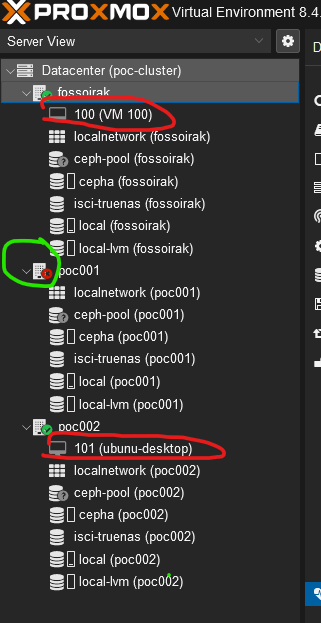
\includegraphics[width=0.55\textwidth]{../poc/failover-prox.png}
  \caption{failover node virtuale machines herstellen in HA in Proxmox VE}
  \label{fig:failover-vm}
\end{figure}

Van zodra de connectie van poc001 verboken is met de nadere nodes duurt het ongeveer 30-60 seconden vooraleer de virtuele machines opnieuw worden opgestart op een andere node. Dit is ook de tijd die nodig is om de heartbeat van de cluster te verliezen.
Hierbij kan ervan uitgegaan worden dat de standaard healthy check van de cluster en zijn nodes ook rond deze tijdsduur ligt. Beide virtuele machines worden opnieuw opgestart op de node foissarak en poc002. \\
Aangezien beide virtuele machines dezelfde HA group hebben, krijgen ze ook dezelfde prioriteit.

Merk op dat zowel de virtuele machine met een SAN als de virtuele machine met een distributed storage opnieuw worden opgestart op de node foissarak. Dit toont aan dat Proxmox VE goed werkt met beide storage systemen, zeker met failover situaties.

\subsection{Virtuele machines migraties in Proxmox VE}
In het het werkveld komt het geregeld voor dat een node een gepland onderhoud heeft. Dit kan zijn dat er een update moet worden uitgevoerd of dat er hardware moet worden vervangen.
Bij deze is het gewenst om te weten of er een mogelijkheid is om de virtuele machines te migreren naar een andere node zonder dat er downtime/minimale downtime is.
Via de GUI in Proxmox VE kan een virtuele machine eenvoudig worden gemigreerd via de optie Migration rechtsboven, zodra een virtuele machine is geselecteerd, zie Figuur \ref{fig:migratie-vm}.
\begin{figure}[H]
  \centering
  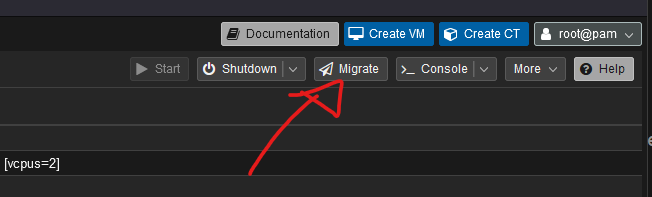
\includegraphics[width=0.85\textwidth]{../poc/vm-migratie-prox.png}
  \caption{migratie virtuele machine in Proxmox VE}
  \label{fig:migratie-vm}
\end{figure}
Tijdens het migreren van de virtuele machine blijft de console open staan van de virtuele machine. Hierbij is er een zeer korte freeze in het beeld waarna de activiteiten in de vm weer verder werken. Het totale proces voor beide virtuele machines individueel was ongeveer 30 seconden.
Hieruit kan er bekeken worden dat de downtime bij migratie zo goed als minimaal is, wat ideaal is voor het offline brengen van een node voor bijvoorbeeld een gepland onderhoud.

\subsection{Hot swapping fysieke disks in Proxmox VE}
Proxmox VE biedt ook hot swapping aan van de fysieke disks. 
Voor deze test is er een fysieke disk voor node poc002 toegevoegd, zie Figuur \ref{fig:hotdisk-swap}.
\begin{figure}[H]
  \centering
  \hspace*{-1cm} % schuift de hele afbeelding 1cm naar links
  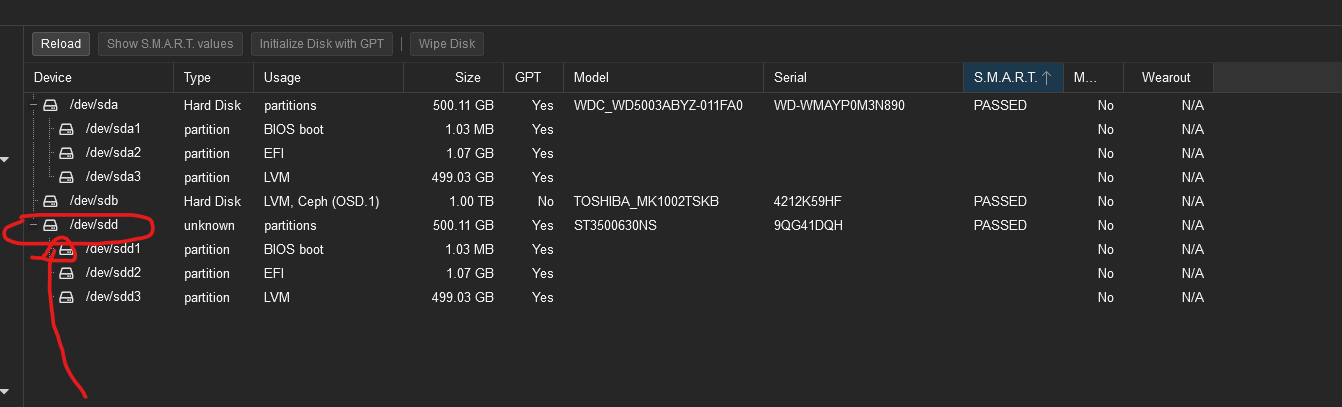
\includegraphics[width=1.1\textwidth, trim=0cm 0cm 15cm 0cm, clip]{../poc/hot-disk-prox.png}
  \caption{Hot disk swap in Proxmox VE met huidige disk}
  \label{fig:hotdisk-swap}
\end{figure}

Deze noemt sdb. Eenmaal dat deze disk is toegevoegd zou de disk moeten kunnen verwijderd worden en vervangen worden door een andere zonder dat de node poc002 offline moet worden gehaald.
Dit wordt live getest tijden het draaien. Op deze disk draait momenteel niks. Hierbij wordt ervan uitgegaan dat het vervangen van een disk wordt gesimuleerd.. De data zou normaal op voorhand moeten verwijderd zijn van de disk.

We voegen de nieuwe disk toe in de plaats van de andere en merken direct na 15 seconden dit op, zie Figuur \ref{fig:hotdiskvervangen-swap}
\begin{figure}[H]
  \centering
  \hspace*{-1cm}
  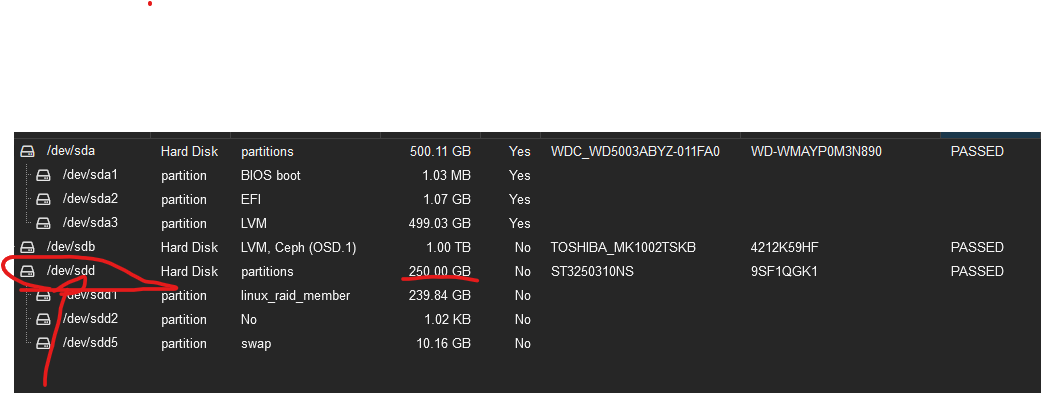
\includegraphics[width=1.1\textwidth, trim=0cm 0cm 10cm 0cm, clip]{../poc/hot-disktwee-prox.png}
  \caption{Hot disk swap in Proxmox VE met nieuwe disk}
  \label{fig:hotdiskvervangen-swap}
\end{figure}


We zien bij Figuur \ref{fig:hotdiskvervangen-swap} dit duidelijk een andere disk is met nu een grote van 250 GB. Hiervoor was dat 500 GB.
% Voor deze virtual managementplatform wordt er Proxmox VE 8.4 gebruikt. Dit is de laatste versie van Proxmox VE die op dit moment beschikbaar is.
% \subsection{cluster opstelling in Proxmox VE}
% Voor proxmox VE is er gekozen om te werken met 3 fysieke node's. Zoals beschreven op de officiële documentatiepagina van Proxmox ondersteunt het platform high availability clustering maar moeten er minimaal 3 nodes in de cluster draaien ~\autocite{proxmoxHA}.
% Hierbij spreken we over minimaal 50\% van de nodes die moeten draaien om de cluster operationeel te houden. Dit is ook de reden waarom er voor 3 nodes is gekozen.
% Bij 2 nodes zou er bij een node failure geen quorum zijn en zou de cluster niet meer operationeel zijn. Dit wil zeggen dat er geen 50\% meerderheid is van de cluster die online is. Enkel bij 3 nodes kan er 1 node uitvallen en alsnog meer dan 50 procent online hebben. In zo een geval spreken we van een quorum.
% In de Figuur \ref{fig:cluster-proxmox} wordt de opstelling getoond. Elke node heeft zijn unieke naam in de cluster, vaak is dat de hostname zelf.
% \begin{figure}[H]
%   \centering
%   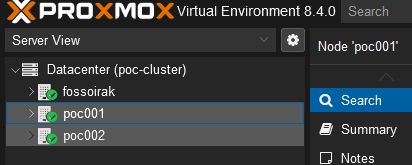
\includegraphics[width=0.85\textwidth]{../poc/cluster-info-prox.png}
%   \caption{Clusteropstelling in Proxmox VE}
%   \label{fig:cluster-proxmox}
% \end{figure}
% \subsection{Storage in Proxmox VE}
% Proxmox VE ondersteunt verschillende soorten storage. In de proof of concept is er gekozen om te werken met een CEPH storage als distributed storage. Dit is een open-source software-defined storage oplossing die kan worden gebruikt in combinatie met Proxmox VE.
% Om deze te configureren moeten er minimaal 3 schijven/partities zijn. Voor deze POC is er besloten om op elke fysieke node een fysieke schijf toe te kennen aan de CEPH storage. Dit zijn 3 willekeurige harde schijven.
% Via de GUI kan vanaf elke node worden doorgeklikt naar Ceph. Daar moet worden aangeduid welke schijf gebruikt zal worden voor de Ceph-storage. Dit kan ook via de command line.
% Nadat de schijven op elke node zijn toegevoegd, kan via het OSD-menu in de Proxmox-GUI een overzicht worden bekeken, zoals te zien is in Figuur \ref{fig:osd-ceph-proxmox}.
% \begin{figure}[H]
%   \centering
%   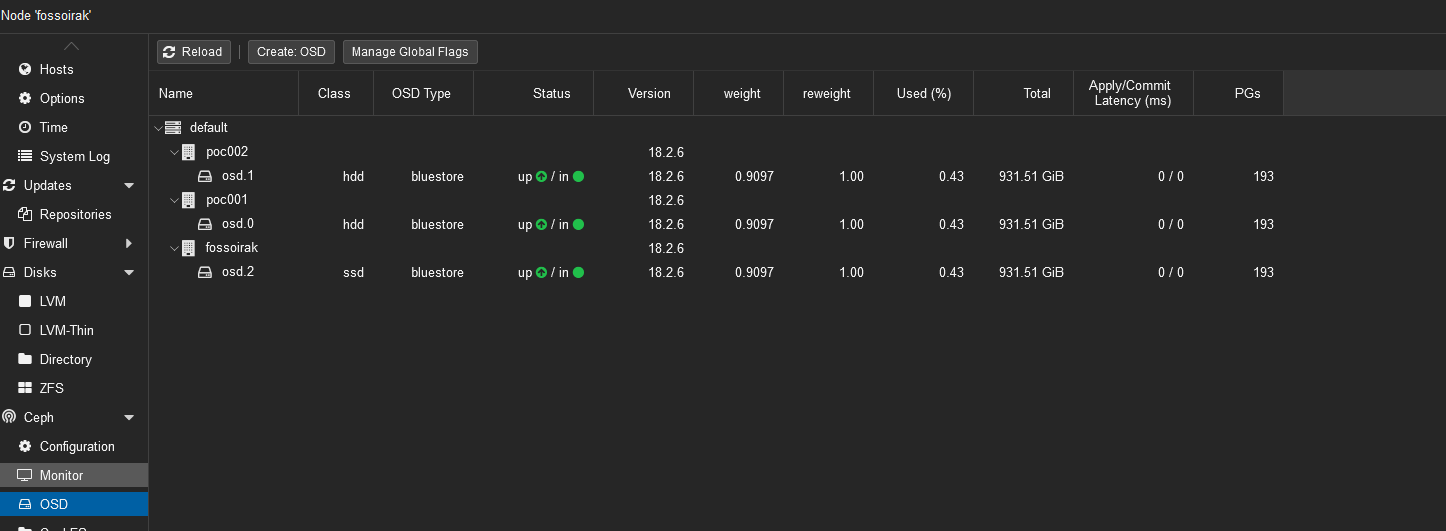
\includegraphics[width=1.2\textwidth]{../poc/ceph-osd-prox.png}
%   \caption{CEPH schijven opstelling in Proxmox VE}
%   \label{fig:osd-ceph-proxmox}
% \end{figure}

% Nu kan er een pool aangemaakt worden voor de CEPH storage. Hierin wordt het belangrijste deel van de CEPH configuratie gedaan.
% Je geeft aan hoeveel schijven er in de pool moeten zitten. Minimaal is dit hier 3 aangezien we weer met het HA systeem zitten. Om de HA regels te volgen is het ook essentieel dat er op elke fysieke node een schijf zit voor de pool.
% Bij het gebruik van Ceph in Proxmox VE moet het systeem weten hoeveel schijven minimaal beschikbaar moeten zijn om de opslagpool operationeel te houden. Voor deze POC wordt dit ingesteld op 2. Dit is ook de reden waarom er met 3 fysieke nodes is gewerkt. Bij een node failure kan de pool nog steeds gebruikt worden.
% De Crush rule in de configuratie is ook belangrijk. Dit is de manier waarop de data verdeeld wordt over de verschillende schijven. Hierin kan ook worden aangegeven dat er een replica van de data op een andere node moet worden gemaakt. Bij een node failure kan de data nog steeds worden benaderd via de andere nodes.
% De firguur \ref{fig:ceph-pool-prox} toont de huidige configuratie van de pool in Proxmox VE.
% \begin{figure}[H]
%   \centering
%   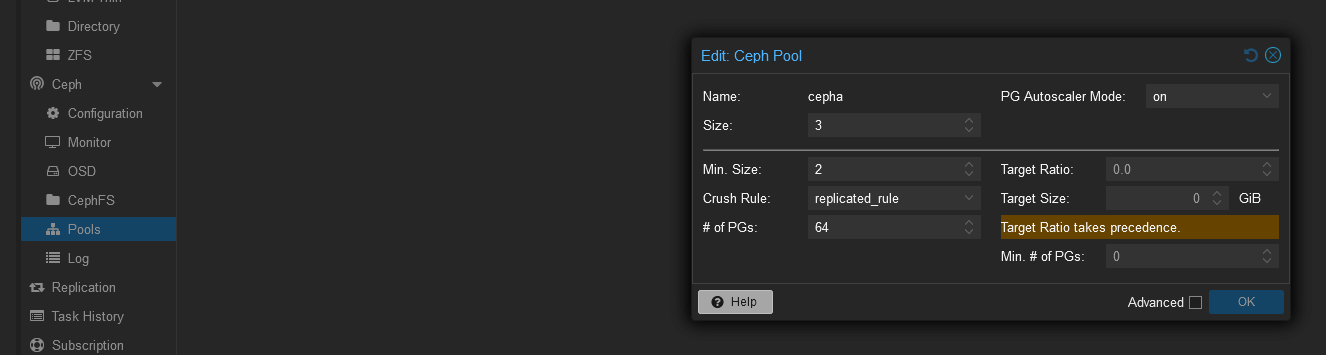
\includegraphics[width=1.1\textwidth]{../poc/ceph-pool-prox.png}
%   \caption{Pool opstelling van CEPH in Proxmox VE}
%   \label{fig:ceph-pool-prox}
% \end{figure}

% Eenmaal aangemaakt kan er een virtuele machine worden aangemakt. Deze virtuele zal Ubuntu 22.04 worden gebruikt als operating system.
% De meeste instellingen kunnen helemaal naar keuze worden ingesteld en is voor de rest buiten de scope van deze bachelorproef. De meest relevante instellingen zijn die rond de storage.
% Tijdens het configureren van de virtuele machine kan de gewenste schijf worden geselecteerd. Hierbij kan ook de eerder aangemaakte pool worden gekozen.
% Merk verder op dat er al een optie is voor SAN iSCSI met TrueNAS~\autocite{truenas} . Deze optie mag tijdelijk genegeerd worden.
% Als alles correct is verlopen, kan op alle drie de nodes naar keuze een virtuele machine worden aangemaakt, waarbij overal dezelfde optie beschikbaar is om Ceph als schijfopslag te gebruiken.
% Figuur \ref{fig:vm-storage-proxmox} toont de configuratie van de virtuele machine in Proxmox VE.
% \begin{figure}[H]
%   \centering
%   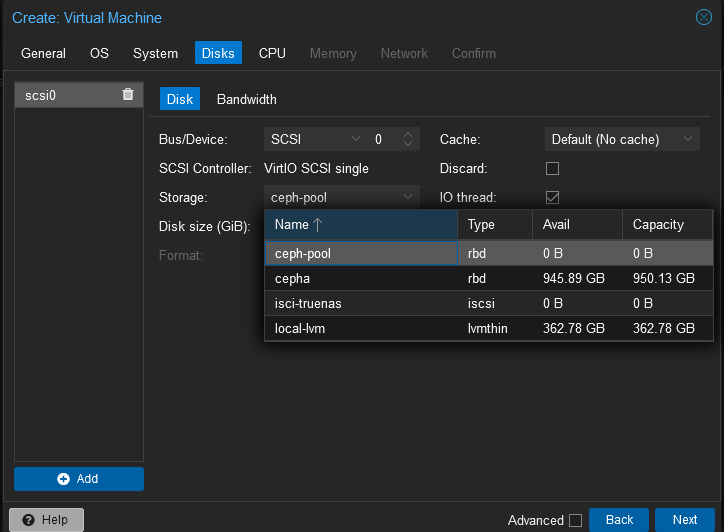
\includegraphics[width=0.85\textwidth]{../poc/vm-storage-prox.png}
%   \caption{VM configuratie met correcte disk in Proxmox VE}
%   \label{fig:vm-storage-proxmox}
% \end{figure}

% De virtuele machine is nu aangemaakt op de node fossoirak.
% Ter controle kan er in de GUI onder Datacenter bij de optie CEPH gekeken worden of alle schijven en nodes die de CEPH pool draaien healthy zijn. Zie figur \ref{fig:ceph-healthy-prox}.
% Als er geen rode kruisjes staan bij de schijven en nodes is alles perfect geconfigureerd.
% \begin{figure}[H]
%   \centering
%   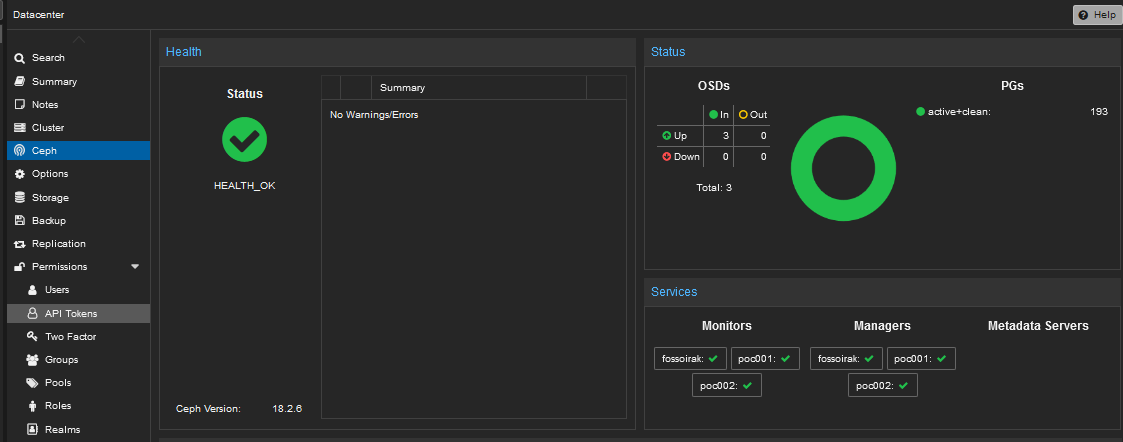
\includegraphics[width=0.85\textwidth]{../poc/ceph-healthy-prox.png}
%   \caption{de gezondheid van CEPH  in Proxmox VE}
%   \label{fig:ceph-healthy-prox}
% \end{figure}

% Hierna kan er een HA test uitgevoerd worden. Dit wordt later besproken.
% Tijdens het werken met Proxmox VE valt er op dat Proxmox VE automatisch een direct attach storage mount aanmaakt voor te gebruiken. Deze wordt gekoppeld als een directory met als naam local.
% Dit toont aan dat Proxmox VE standaard een integratie biedt met DAS. In deze situatie draait het direct op de schijf waar de Proxmox VE zelf op draait zoals te zien is in de Figuur \ref{fig:das-prox}.
% \begin{figure}[H]
%   \centering
%   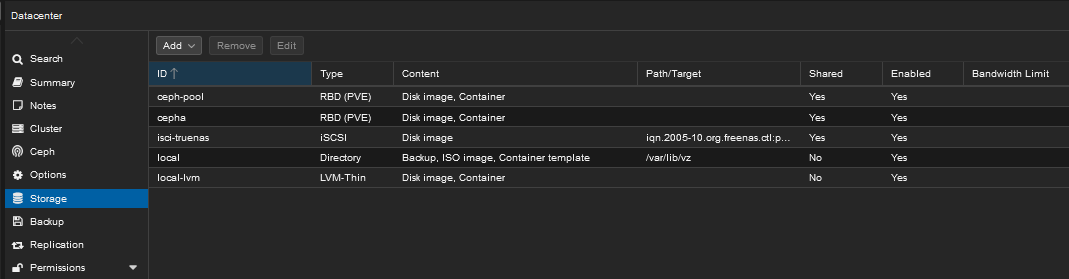
\includegraphics[width=1.1\textwidth]{../poc/das-proxmox.png}
%   \caption{direct attach storage in Proxmox VE}
%   \label{fig:das-prox}
% \end{figure}


% Nu we weten dat CEPH goed werkt moet er gekeken worden naar de SAN configuratie met ISCSI.
% Er is een bestaande TrueNAS ~\autocite{truenas} server die al draait in de omgeving. Hierop draait een block storage waar iSCI is geconfigureerd.
% Onder de tab storage bij Datacenter kan er zeer eenvoudig een iSCSI target worden aangemaakt bij Add, zie Figuur \ref{fig:iscsi-SAN}.
% Via de opties in het menu moet er een correct ID als naam worden gegeven en via portal het correct IP adres van de TrueNAS service.
% Omdat er gewerkt wordt met een SAN principe staat het default bij de optie node in de configuratie op all nodes. Dit is ook de bedoeling aangezien we met een HA cluster werken.
% De configuratie van iSCI op TrueNAS is buiten de scope van deze bachelorproef.
% \begin{figure}[H]
%   \centering
%   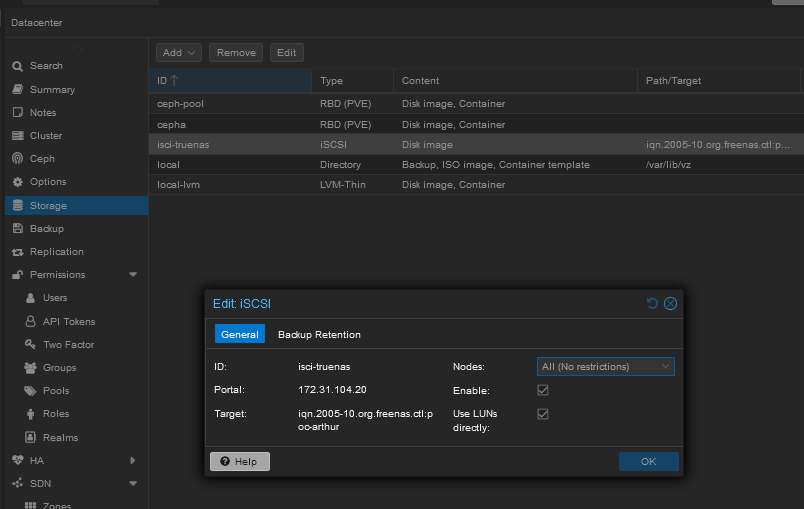
\includegraphics[width=0.85\textwidth]{../poc/iscsi-prox.png}
%   \caption{storage area network met ISCI in Proxmox VE}
%   \label{fig:iscsi-SAN}
% \end{figure}
% Nu zal er een extra  optie bijgekomen zijn in de GUI onder de tab storage bij datacenter, zie fiuur~\ref{fig:vm-lijst}  Hier in het voorbeeld wordt het al naam iSCI-TrueNAS gegeven.
% Nu maken we een 2de virtuele machine aan met dezelfde configuratie als de eerste virtuele machine maar met een andere disk. Er wordt nu gekozen voor de isci-truenas disk.
% \begin{figure}[H]
%   \centering
%   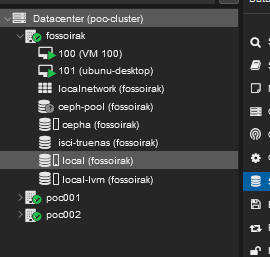
\includegraphics[width=0.85\textwidth]{../poc/vm-lijst-prox.png}
%   \caption{Lijst van de 2 virtuele machines in Proxmox VE}
%   \label{fig:vm-lijst}
% \end{figure}
% Aangezien een SAN princiepe via een vebrinding werkt op het netwerk is de storage de zwakste schakel in een high availability cluster. Deze verbinding kan verbroken worden door netwerk problemen. Hierna kan er data corruptie onstaan in het slechtste geval.

% \subsection{High Availability in Proxmox VE}

% Eenmaal de storage in orde is voor de virtuele machines kan er een HA configuratie worden aangemaakt. 
% Onder datacenter HA kan een groep worden aangemaakt. Hierin worden alle drie de fysieke nodes opgenomen die deel uitmaken van de cluster. Vervolgens wordt aan de groep een logische naam toegekend, in dit geval ha-pool zoals in Figuur \ref{fig:ha-group}.
% \begin{figure}[H]
%   \centering
%   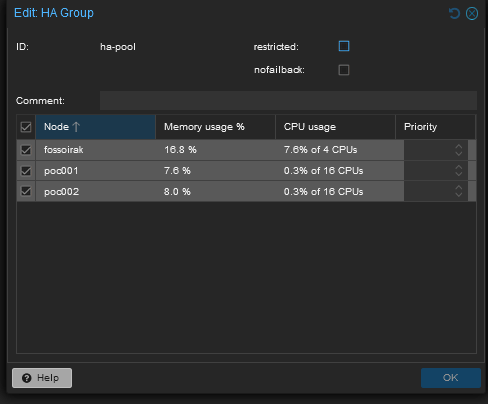
\includegraphics[width=0.85\textwidth]{../poc/ha-group.png}
%   \caption{high Availability group in Proxmox VE}
%   \label{fig:ha-group}
% \end{figure}
% Nu voegen we de 2 virtuele machines toe aan de HA groep. Dit wordt gedaan via de HA section in datancer.
% Bij Max Restart en Max Relocate wordt ingesteld hoe vaak een virtuele machine opnieuw mag worden opgestart of verplaatst naar een andere node. In dit geval moet dit groter zijn dan 0 zoals bij firguur \ref{fig:ha-vm}.
% \begin{figure}[H]
%   \centering
%   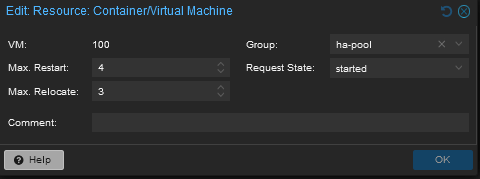
\includegraphics[width=0.85\textwidth]{../poc/vm-ha.png}
%   \caption{High Availability vm toevoegen in Proxmox VE}
%   \label{fig:ha-vm}
% \end{figure}
% Zodra beide virtuele machines aan de HA-groep zijn toegevoegd, kan de HA-configuratie worden getest.

% Om HA te testen in combinatie met beide storage systemen zal er een netwerk probleem worden gesimuleerd.
% Alle virtuele machines draaien nu op node 001
% Op de fysieke node poc001 zal de internet kabel worden uitgetrokken. Hierna kijken we hoelang het duurt vooraleer de virtuele machines opnieuw worden opgestart op een andere node, alsookop welke node specifiek.

% Figuur \ref{fig:failover-vm} kan er duidelijk gezien worden dat de virtuele machines volledig van cold mode moeten opstarten. Dit is een andere situatie dan wanneer er een migratie gedaan wordt.
% Dan wordt live de virtuele machine van de ene node naar de andere gemigreerd zonder echte downtime.
% Het systeem in Proxmox VE is nu zo ingesteld dat bij een echte failover de schade van downtime relatief beperkt blijft. Dit staat uiteraard los van data verlies die kan optreden bij een failover.
% \begin{figure}[H]
%   \centering
%   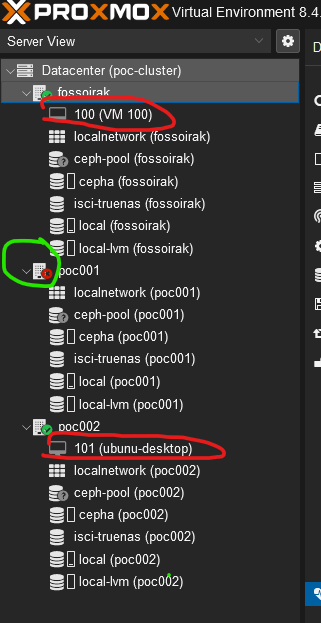
\includegraphics[width=0.85\textwidth]{../poc/failover-prox.png}
%   \caption{failover node virtuale machines herstellen in HA in Proxmox VE}
%   \label{fig:failover-vm}
% \end{figure}

% Van zodra de connectie van poc001 verboken is met de nadere nodes duurt het ongeveer 30-60 seconden vooraleer de virtuele machines opnieuw worden opgestart op een andere node. Dit is ook de tijd die nodig is om de heartbeat van de cluster te verliezen.
% Hierbij kunenn we vanuit gaan dat de default healthy check van de cluster en zijn nodes ook rond deze tijdsduur ligt. Beide virtuele machines worden opnieuw opgestart op de node foissarak en poc002. 
% Aangezien beide virtuele machines dezelfde HA group hebben, krijgen ze ook dezelfde prioriteit.

% Merk op dat zowel de virtuele machine met een SAN als de virtuele machine met een distributed storage opnieuw worden opgestart op de node foissarak. Dit toont aan dat Proxmox VE goed werkt met beide storage systemen, zeker met failover situaties.


% \subsection{Virtuele machines migraties in Proxmox VE}
% In het het werkveld komt het geregeld voor dat een node een gepland onderhoud heeft. Dit kan zijn dat er een update moet worden uitgevoerd of dat er hardware moet worden vervangen.
% Bij deze is het gewenst om te weten of er een mogelijkheid is om de virtuele machines te migreren naar een andere node zonder dat er downtime/minimale downtime is.
% Via de GUI in Proxmox VE kan een virtuele machine eenvoudig worden gemigreerd via de optie Migration rechtsboven, zodra een virtuele machine is geselecteerd, zie Figuur \ref{fig:migratie-vm}.
% \begin{figure}[H]
%   \centering
%   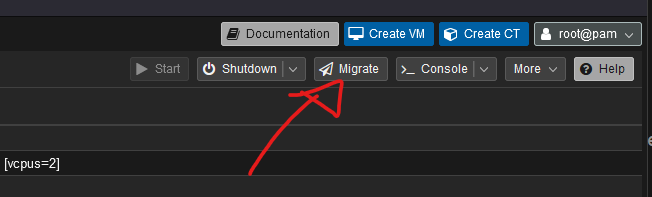
\includegraphics[width=0.85\textwidth]{../poc/vm-migratie-prox.png}
%   \caption{migratie virtuele machine in Proxmox VE}
%   \label{fig:migratie-vm}
% \end{figure}
% Tijdens het migreren van de virtuele machine blijft de console open staan van de virtuele machine. Hierbij is er een zeer korte freeze in het beeld waarna de activiteiten in de vm weer verder werken. Het totale proces voor beide virtuele machines individueel was ongeveer 30 seconden.
% Hieruit kan er bekeken worden dat de downtime bij migratie zo goed als minimaal is, wat ideaal is voor het offline brengen van een node voor bijvoorbeeld een gepland onderhoud.


% \subsection{Hot swapping fysieke disks in Proxmox VE}
% Proxmox VE biedt ook hot swapping aan van de fysieke disks. 
% Voor deze test is er een fysieke disk voor node poc002 toegevoegd, zie Figuur \ref{fig:hotdisk-swap}.
% \begin{figure}[H]
%   \centering
%   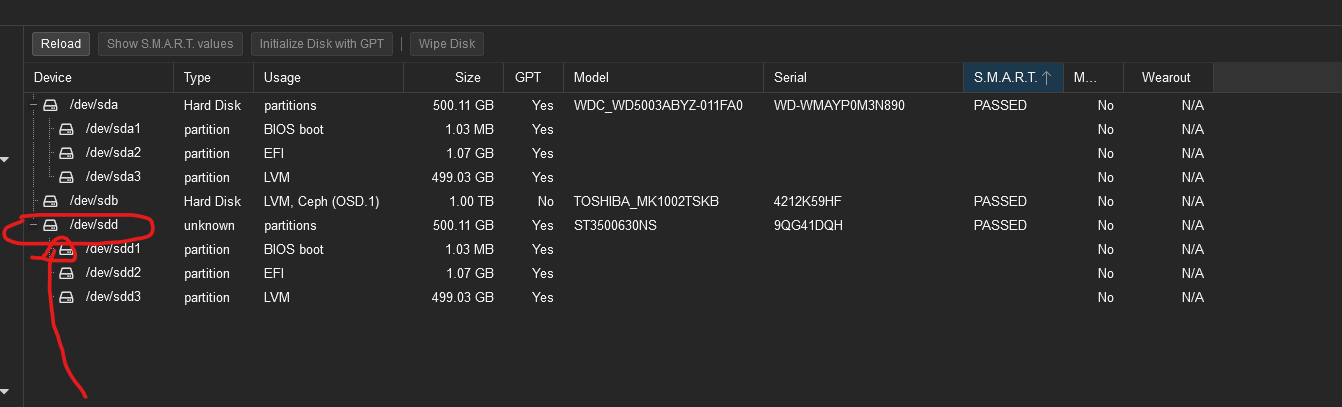
\includegraphics[width=1.2\textwidth]{../poc/hot-disk-prox.png}
%   \caption{hot disk swap in Proxmox VE}
%   \label{fig:hotdisk-swap}
% \end{figure}
% Deze noemt sdb. Eenmaal dat deze disk is toegevoegd zou de disk moeten kunnen verwijderd worden en vervangen worden door een andere zonder dat de node poc002 offline moet worden gehaald.
% Dit wordt live getest tijden het draaien. Op deze disk draait momenteel niks. Dit is belangrijk aangezien we het vervangen van een disk simuleren. De data zou normaal op voorhand moeten verwijderd zijn van de disk.

% We voegen de nieuwe disk toe in de plaats van de andere en merken direct na 15 seconden dit op, zie Figuur \ref{fig:hotdiskvervangen-swap}.
% \begin{figure}[H]
%   \centering
%   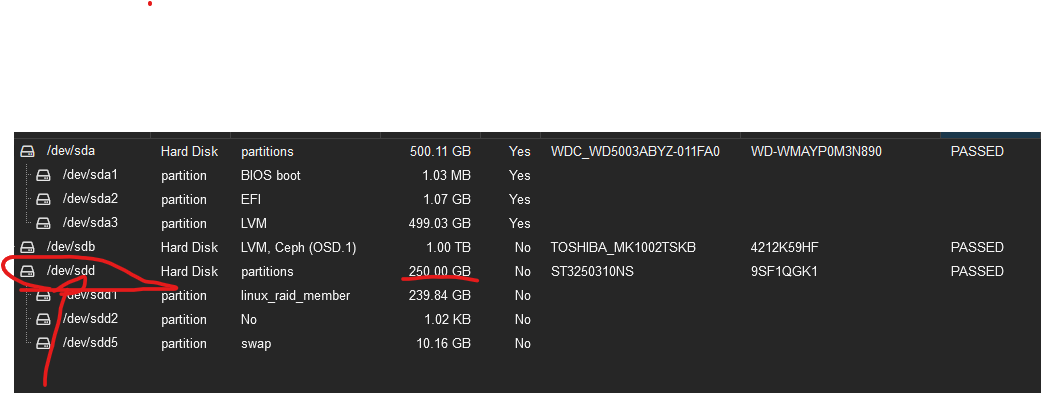
\includegraphics[width=1.2\textwidth]{../poc/hot-disktwee-prox.png}
%   \caption{hot disk swap in Proxmox VE}
%   \label{fig:hotdiskvervangen-swap}
% \end{figure}

% We zien bij Figuur \ref{fig:hotdiskvervangen-swap} dit duidelijk een andere disk is met nu een grote van 250 GB. Hiervoor was dat 500 GB.


\section{Xen Orchestra}%
Deze software wordt gedraaid in combinatie met de hypervisor XCP-ng versie 8.3. Dit is de laatste versie van XCP-ng die op dit moment beschikbaar is en als stabiel kan worden beschouwd.  
Xen Orchestra zal draaien in een virtuele machine op een van de fysieke nodes van de cluster. Xen Orchestra zelf draait op versie 5.106.  
De keuze is gemaakt om de enterprise trial-licentie te activeren, aangezien deze meer features ter beschikking heeft dan de communityversie. Meer specifiek biedt de enterpriseversie ook een ingebouwde ondersteuning voor een distributed storage-systeem, XOSTOR.

\subsection{Storage in Xen Orchestra}%
Zoals eerder vermeld moeten er twee soorten storagesystemen worden getest. Deze moeten het mogelijk maken om virtuele machines te kunnen draaien in een High Availability-methode.  
Xen Orchestra biedt zowel SAN-integratie als ook een distributed storage-integratie aan.  
De volgende twee storagesystemen worden specifiek getest.

\begin{itemize}
    \item XOSTOR storage~\autocite{vates_xostor}, is een implementatie van een distributed storage-systeem dat volledig draait over de cluster heen als virtuele SAN (VSAN).
    \item SAN iSCSI (met TrueNAS~\autocite{truenas})
\end{itemize}
In sectie \nameref{sec:storage_orch} wordt er dieper ingegaan op de configuratie van de storage in Xen Orchestra.  
XOSTOR wordt toegepast op alle drie de fysieke nodes. Elk heeft zijn eigen schijf die gebruikt wordt door XOSTOR. Deze schijven nemen elkaars taken over bij een failover of het maken van redundante data.  
iSCSI bij Xen Orchestra biedt op een makkelijke manier de mogelijkheid om een SAN te configureren.  
Elke storageoptie krijgt een virtuele machine toegewezen om de storage te testen en te bekijken of deze correct werkt.  
Uiteindelijk worden beide virtuele machines probleemloos aangemaakt met hun eigen storagetoepassing. Zie \ref{fig:virtuelemachines-orch} voor meer details.

\subsection{High Availability in Xen Orchestra}%
Momenteel zijn er twee virtuele machines aangemaakt in Xen Orchestra. Deze zijn respectievelijk verbonden met de XOSTOR- en de iSCSI-storage.  
Nu is er nog geen sprake van een High Availability-principe. Hiervoor moet de cluster extra configuratie krijgen om bij een eventuele node failure de virtuele machines opnieuw te kunnen opstarten op een andere node.  
Zie \nameref{sec:ha-orch} voor de specifieke configuratie van de HA in Xen Orchestra.

Om een realistische test te doen waarbij het HA-principe kan worden getest, zal er een node failure worden gesimuleerd.  
Dit wordt gedaan door een netwerkkabel fysiek uit te trekken uit de node waar beide virtuele machines op draaien.  
Het duurt tot maximaal 70 seconden vooraleer Xen Orchestra ingrijpt en ziet dat er een node offline is. Hierna start Xen Orchestra onmiddellijk met het starten van de virtuele machines op een andere node die healthy is en voldoende resources over heeft.  
Figuur \ref{fig:failure-orch} toont duidelijk dat Xen Orchestra de virtuele machines opnieuw opstart op een andere node. Dit is een cold start aangezien de virtuele machines volledig opnieuw moeten worden opgestart.

\begin{figure}[H]
  \centering
  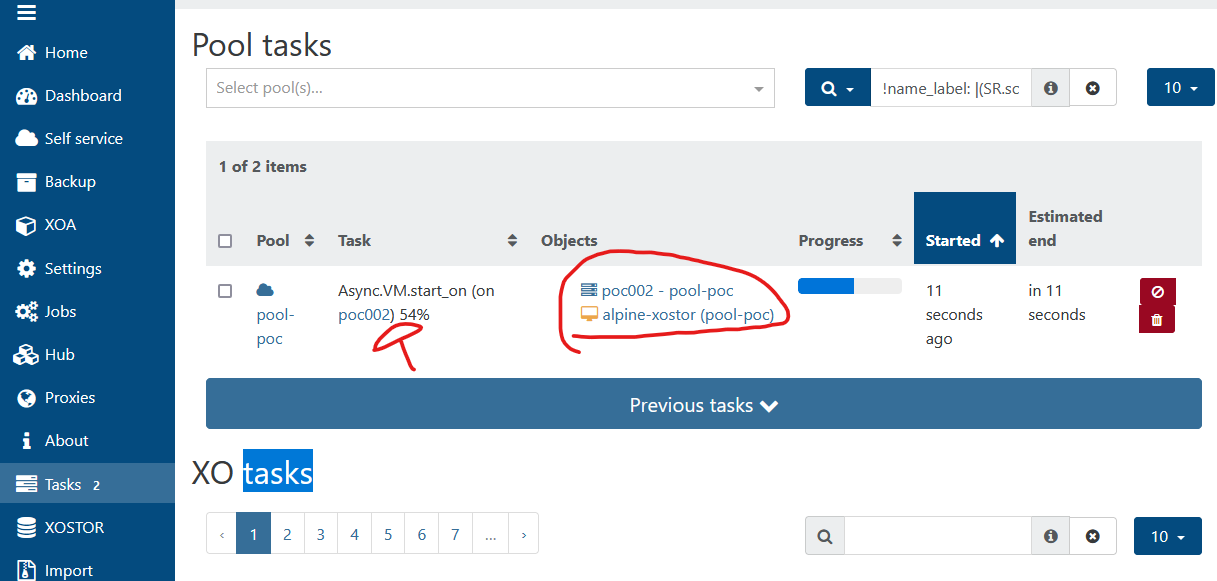
\includegraphics[width=1.1\textwidth, trim=0cm 0cm 5cm 0cm, clip]{../poc/failure-orch.png}
  \caption{Failover: node, virtuele machines herstellen in HA in Xen Orchestra}
  \label{fig:failure-orch}    
\end{figure}
Tijdens de overgang valt de verbinding met de virtuele machine volledig weg. Dit is te wijten aan het feit dat de virtuele machines volledig opnieuw moeten worden opgestart, zoals eerder vermeld.

\subsection{Virtuele machines migraties in Xen Orchestra}%
Nu HA getest is met failover-situaties, moet ook geweten worden hoe HA kan worden toegepast bij een gepland onderhoud. Dit wil zeggen dat er 0 downtime gewenst is, maar dat er tegelijkertijd wel aan een node gewerkt kan worden.
In deze proof of concept wordt dit specifiek getest door de twee virtuele machines te laten draaien op een node die bewust offline wordt gehaald.
Hierna worden beide virtuele machines naar een andere willekeurige node gemigreerd. Tijdens de migratie wordt gekeken of de virtuele machine afwijkend gedrag vertoont tijdens het migreren.
Beide virtuele machines draaien nog steeds op node poc002. Tegelijkertijd wordt een migratiecommando uitgevoerd.
De informatie die Xen Orchestra nodig heeft om de migratie uit te kunnen voeren, wordt ingegeven. Hierbij wordt dezelfde storageoptie meegegeven die de virtuele machine nu heeft. Enkel de target host verandert. (Zie Figuur \ref{fig:migratie-vm-orch}).

\begin{figure}[H]
  \centering
  \hspace*{-1cm}  
  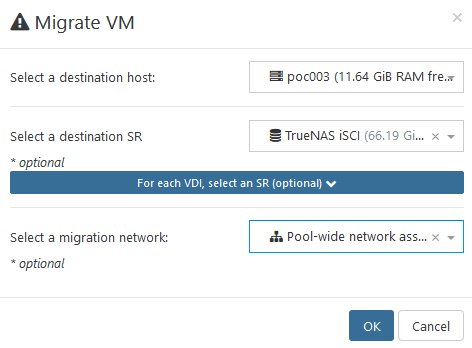
\includegraphics[width=0.9\textwidth]{../poc/migratie-vm-orch.png}
  \caption{Migratie virtuele machine in Xen Orchestra}
  \label{fig:migratie-vm-orch}
\end{figure}

In Figuur \ref{fig:migratie-proces-orch} is te zien dat de migratie wordt uitgevoerd. De virtuele machine blijft volledig bereikbaar tijdens de migratie. Er wordt enkel een kleine hapering van 5 seconden opgemerkt bij de SAN-storage met iSCSI.  
In Figuur \ref{fig:migratie-proces-orch} is ook te zien dat XOSTOR-storage veel sneller migreert dan SAN met iSCSI. Wellicht is dit te wijten aan het feit dat het netwerk de bottleneck is bij iSCSI.

\begin{figure}[H]
  \centering
  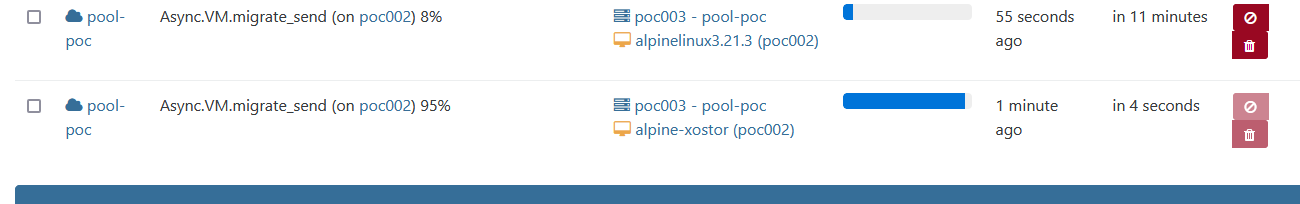
\includegraphics[width=1.1\textwidth]{../poc/migratie-proces-orch.png}
  \caption{Migratieproces in Xen Orchestra}
  \label{fig:migratie-proces-orch}  
\end{figure}


\subsection{Hot swapping fysieke disks in Xen Orchestra}%
Bij dit gedeelte van de proof of concept is het belangrijk dat een kapotte schijf vervangen kan worden zonder dat de node offline gehaald hoeft te worden.
In dit geval wordt ervan uitgegaan dat alle data al van de disk gehaald is en klaar is voor vervanging.
De disk wordt uit de fysieke node gehaald en vervangen door een andere, waarna gekeken wordt of de disk teruggevonden kan worden in Xen Orchestra.
Aangezien Xen Orchestra zelf geen diskmanagement heeft, moet met SSH worden verbonden op de specifieke node waar de disk is vervangen. Daar kan op de reguliere manier een disk worden gemount en gepartitioneerd.
Hierna kan de disk worden toegevoegd aan Xen Orchestra als een storageoptie. In de GUI moet dan het correcte pad worden toegevoegd (Zie Figuur~\ref{fig:storage-path-orch}). Er wordt opgemerkt dat dit een extra stap is die moet gebeuren.

\begin{figure}[H]
  \centering
  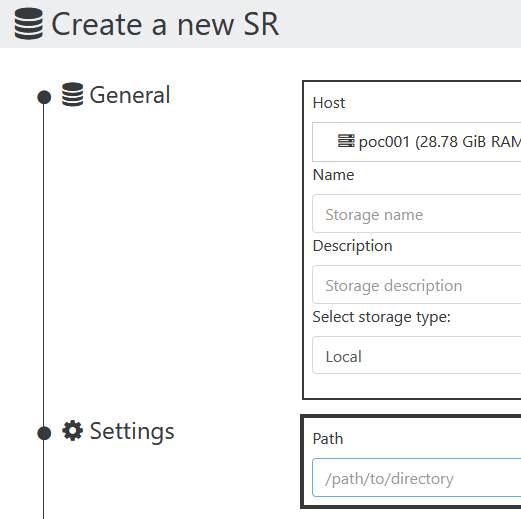
\includegraphics[width=0.8\textwidth]{../poc/storage-path-orch.png}
  \caption{Storagepad configuratievoorbeeld in Xen Orchestra}
  \label{fig:storage-path-orch}  
\end{figure}
\section{XenCenter}%
XenCenter is het volgende virtual managementplatform die getest wordt. Deze applicatie zal samen gedraaid worden met Citrix Hypervisor (XenServer).
3 fysieke nodes zullen elk de XenServer-installatie krijgen. XenCenter dient geïnstalleerd te worden op een Windows-machine als app.
Zowel de hypervisor als XenServer draaien op de laatste beschikbare versie. XenServer heeft momenteel versie 8.4 en XenCenter heeft de versie 2025.2.0.
Er wordt een pool aangemaakt waar de virtuele machines in zitten zoals in Figuur \ref{fig:opstel-xen}.
In \nameref{sec:Clusteropstelling-Xen} wordt de opstelling in meer detail uitgelegd.
\begin{figure}[H]
\centering
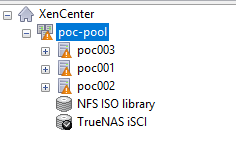
\includegraphics[width=0.8\textwidth]{../poc/opstel-xen.png}
\caption{Basis opstelling voor XenCenter}
\label{fig:opstel-xen}
\end{figure}

\subsection{Storage in XenCenter}%
Er moet ook getest worden hoe virtual managementplatformen omgaan met gebruik van SAN iSCSI en distributed storage systemen.
XenCenter biedt standaard een built-in systeem voor SAN storage te koppelen aan een cluster met iSCSI als protocol.
Verder binnen de XenCenter-applicatie is er geen directe ondersteuning mogelijk voor distributed storage systemen zoals CEPH~\autocite{weil2006ceph} of XOSTOR bij Xen Orchestra.
Er bestaan workarounds om systemen zoals CEPH te gebruiken, helaas zijn deze niet officieel ondersteund door XenCenter. Hierdoor kan er ook geen beroep worden gedaan op officiële support van het bedrijf bij problemen, wat wel een must is voor Excentis.
Hierdoor is er geen mogelijkheid om distributed storage te gaan implementeren met XenCenter in deze proof of concept. DAS wordt door elke virtual managementplatform goed ondersteund en is een basis voor elk systeem.
Het biedt alleen geen goede oplossing als we willen werken met een High Availability-principe.
Het volgende wordt getest en bekeken:
\begin{itemize}
\item SAN iSCSI (met TrueNAS~\autocite{truenas})
\end{itemize}
In \nameref{sec:Storage-technisch-xen} wordt de opstelling van de storage en technische instellingen besproken in meer detail.
Het is belangrijk dat er op een correcte goede manier storage kan worden toegevoegd. Hierbij biedt XenCenter een goede duidelijke manier aan om iSCSI-storage toe te voegen.
De iSCSI-target wordt gehost op een TrueNAS~\autocite{truenas} server. Deze instellingen worden verder niet in detail besproken.
Na het instellen van de TrueNAS via iSCSI wordt deze door XenCenter duidelijk weergegeven in het overzichtsmenu, zie Figuur \ref{fig:truenasinlijst-xen}.
\begin{figure}[H]
\centering
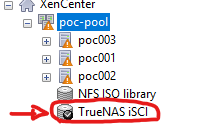
\includegraphics[width=0.8\textwidth]{../poc/truenasinlijst-xen.png}
\caption{iSCSI SAN na configuratie van storage in XenCenter}
\label{fig:truenasinlijst-xen}
\end{figure}

\subsection{High Availability in XenCenter}%
De configuratie voor het opzetten van een High Availability-cluster wordt uitgelegd in \nameref{sec:HA-xen}.
Nu de HA-configuratie aangemaakt is, willen we testen of de High Availability-integratie effectief werkt. Dit wordt gedaan door een fysieke node offline te brengen door een netwerkkabel uit de cluster te halen.
Hierna wordt er gekeken hoelang het duurt voor XenCenter dit detecteert en wat het dan specifiek zal doen om het probleem op te lossen.

Eenmaal de kabel uit de server is gehaald, duurt het ongeveer 1-2 minuten voor XenCenter dit detecteert. Dit is vergelijkbaar met de tijd die XenOrchestra met XCP-ng nodig heeft.
Direct wanneer XenCenter de melding maakt dat er een node offline is waar een virtuele machine op draait, zoekt het naar een nieuwe node om de virtuele machine te kunnen opstarten.
Figuur \ref{fig:failover-xen} toont dit duidelijk aan wat XenCenter dan probeert te doen. Het totale proces duurt maximaal 3 minuten voor de virtuele machine weer opgestart wordt op een andere beschikbare node.
\begin{figure}[H]
\centering
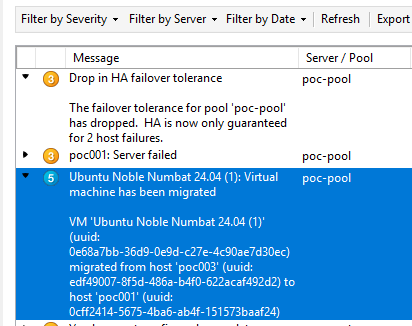
\includegraphics[width=0.8\textwidth]{../poc/failover-xen.png}
\caption{Failover XenCenter activiteiten}
\label{fig:failover-xen}
\end{figure}

\subsection{Virtuele machines migraties in XenCenter}%
Een migratie van een virtuele machine is belangrijk met het oog op dat wanneer er een onderhoud is, geen enkele virtuele machine een downtime heeft.
Hierbij moet er worden nagegaan of XenCenter een implementatie biedt om virtuele machines te migreren zonder een echte downtime van die virtuele machine.
Via XenCenter kan er eenvoudig via de ingebouwde GUI een migratie gestart worden door aan te geven wie de nieuwe target host is.
Vervolgens begint XenCenter met het migratieproces waarbij de connectie van de virtuele machine maximaal 5 seconden wegvalt.
Dit moment is wanneer het laatste stukje data van de oude node naar de nieuwe gaat en de virtuele machine even geen data kan ophalen of wegschrijven.
De duurtijd is vergelijkbaar met de andere virtuele managementplatformen, waarbij het migratieproces voor de eenvoudige virtuele machine ongeveer 3 minuten duurde.
Figuur \ref{fig:migrate-vm-xen} toont hoe de migratie gestart kan worden.
\begin{figure}[H]
\centering
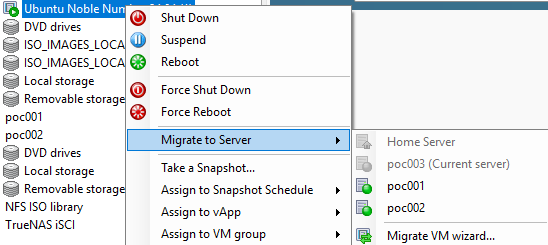
\includegraphics[width=0.8\textwidth]{../poc/migrate-vm-xen.png}
\caption{Migratie starten van virtuele machine in XenCenter}
\label{fig:migrate-vm-xen}
\end{figure}

\subsection{Hot swapping fysieke disks in XenCenter}%
Als er een oude schijf vervangen moet worden of een nieuwe schijf moet worden toegevoegd, is het belangrijk dat deze op een eenvoudige manier te zien is in de GUI van de software.
In dit geval biedt XenCenter geen directe manier om de schijven weer te geven in de applicatie. Er moet manueel ingelogd worden via de console of via SSH op de fysieke node waar de schijf vernieuwd is.
Hierna moet de schijf geformatteerd worden en een EXT4-partitie krijgen via GPT om te kunnen worden uitgelezen in de GUI van XenCenter.
Het kan gebeuren bij verouderde apparatuur dat een restart van het systeem noodzakelijk is voor XenCenter de wijzigingen ziet.
Als alles correct verloopt, moet de storage zichtbaar zijn binnen XenCenter, zie Figuur \ref{fig:swap-storage-xen}.
\begin{figure}[H]
\centering
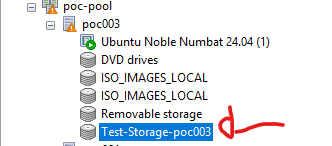
\includegraphics[width=0.8\textwidth]{../poc/swap-storage-xen.png}
\caption{Nieuwe schijf als storage in XenCenter}
\label{fig:swap-storage-xen}
\end{figure}